
\newquestion{Pregunta 2}
Usted trabaja en el diseño de un \emph{sensor en silicio} que, en su etapa de proceso, se modela como una pastilla 1D formada inicialmente por dos regiones tipo \(n\) con dopajes distintos. Para esta etapa
:
  \textbf{Use:}
  \begin{itemize}
    \item $T=300~\mathrm{K}$ $(V_T=\tfrac{k_BT}{q}=0{,}0258~\mathrm{V})$
    \item $\varepsilon_s \approx 1{,}0\times10^{-12}~\mathrm{F/cm}$
    \item $q=1{,}6\times10^{-19}~\mathrm{C}$
    \item $N_{D1}=10^{16}~\mathrm{cm^{-3}}$
    \item $N_{D2}=10^{14}~\mathrm{cm^{-3}}$
    \item $n_i=10^{10}~\mathrm{cm^{-3}}$
  \end{itemize}
  \begin{figure}
  \centering
  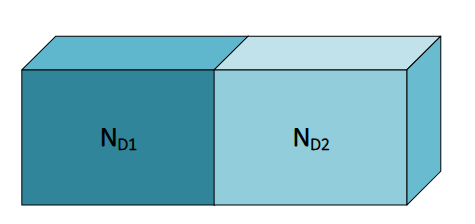
\includegraphics[width=0.5\linewidth]{img/P1_2.png}
  \captionof{figure}{Pastilla de silicio tipo $n\!-\!n$ en equilibrio térmico.}
  \label{fig:nnpastilla}
  \end{figure}
Más adelante, el lado derecho se \emph{redopa a tipo \(p\)} para formar una juntura abrupta \(p\!-\!n\); en ese caso, \textbf{use:}
\begin{itemize}
  \item \(N_A=10^{17}~\mathrm{cm^{-3}}\) (manteniendo \(N_{D2}=10^{14}~\mathrm{cm^{-3}}\))
  \item \(n_i=1{,}12\times10^{10}~\mathrm{cm^{-3}}\) (lado \(p\))
\end{itemize}
En caso de utilizar cualquier aproximación justifíquela claramente.
 


\begin{enumerate}
  \item \textbf{[2 pt]}\;
  Usando tanto las corrientes de difusión como de deriva y usando la relación de Einstein obtenga la expresion dada en \eqref{eq:potenciala} ademas analice los diferentes casos dados por:
  \(N_{D1}>N_{D2}\), \(N_{D2}>N_{D1}\) y \(N_{D1}=N_{D2}\).
  Exprese su resultado como
  \begin{equation}
    V(x_2)-V(x_1)=V_T\ln\!\frac{n(x_2)}{n(x_1)}
    \label{eq:potenciala}
  \end{equation}
  Indique además \emph{en qué lado el potencial es mayor} en cada caso.

  \item \textbf{[1 pt]}\;
  Tras redopar el lado derecho a \(p\) (\(N_A=10^{17}~\mathrm{cm^{-3}}\), \(N_{D2}=10^{14}~\mathrm{cm^{-3}}\)),
  calcule el voltaje  \(V_0\), el ancho total de agotamiento \(L=W=x_n+x_p\) y el campo eléctrico máximo
  \[
  V_0 = V_T\ln\!\left(\frac{p_{p0}}{p_{n0}}\right),\qquad
  L=\sqrt{\frac{2\,|V_0|\,\varepsilon_s}{q}\!\left(\frac{1}{N_A}+\frac{1}{N_D}\right)},\qquad
  E_{\max}=\frac{2\,|V_0|}{L}.
  \]
  Bosqueje el \emph{diagrama de bandas} en equilibrio.
  \begin{figure}
    \centering
    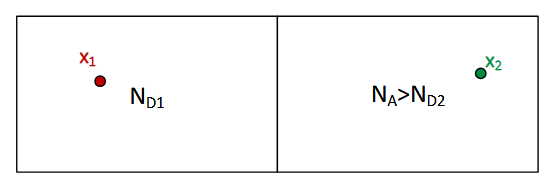
\includegraphics[width=0.6\linewidth]{img/P1_9.png}
    \caption{Diagrama de bandas en equilibrio.}
    \label{fig:bandas_eq}
  \end{figure}
  \item \textbf{[3 pt]}\; Determine y grafique la concentración de portadores a ambos lados de la pastilla, el diagrama de concentraciones, el campo eléctrico en la zona de transición, el potencial eléctrico a lo largo de la pastilla.
\end{enumerate}



